\documentclass[11pt]{article}
\usepackage[utf8]{inputenc}
\usepackage{xeCJK}
\usepackage{geometry}
\usepackage{pifont}
\usepackage{longtable}
\usepackage{booktabs}
\usepackage{float}
\usepackage{makecell}
\usepackage{multirow}
\usepackage{color}
\usepackage{natbib}
\usepackage{graphicx}
\usepackage{bm}
\usepackage{amsmath, amssymb, mathtools}
\usepackage{indentfirst}
\usepackage{caption}
\usepackage[table]{xcolor} % 引入xcolor包
\usepackage{tabularx}
\usepackage{xltabular}
\captionsetup[figure]{name={图}}
\captionsetup[table]{name={表}}
\geometry{top = 1.5cm, bottom = 1.5cm, left = 2.5cm, right = 2.5cm}
\renewcommand{\baselinestretch}{1.4}
\title{\textbf{Group Report - Quantitative Finance}\\
\textit{An Empirical Study on Fundamental Alphas and Aggregations} \footnote{本报告的git仓库地址: https://github.com/Silkdust/quant424}}
\author{\Large 毛思文$^{(1)}$, 涂孟泽$^{(2)}$, 王若妍$^{(3)}$, 张思成$^{(4)}$, 郑婉$^{(5)}$  \footnote{按姓氏音序排列.} \\
   ID: $^{(1)}$2201211276 $^{(2)}$2201211283 $^{(3)}$2201211288 $^{(4)}$2201211308 $^{(5)}$2201211314}
\date{4/24/2023}

\begin{document}
\maketitle

\noindent
\rule[0.2\baselineskip]{\textwidth}{1pt}
        \large \textbf{摘要:  }\normalsize 使用多因子策略进行量化投资时,因子合成是提取多维度因子信息的重要方式之一,也是因子选股的重要环节。本研究选取了31个代表性的基本面因子,尝试了七种因子组合方式,包括等权组合、历史收益率加权、历史IC加权、最大化ICIR、最大化IC、主成分分析和神经网络等方法,综合比较了去除Barra风格因子和行业因子前与去除后的组合表现。随后,本研究利用上述因子组合在A股市场构建了多空选股策略,最终得到了回测期(2016年1月至2022年12月)内的稳健型和进取型两种策略,取得高于基准的夏普比率和年化收益率。
        
        \noindent
        \large \textbf{关键词:  }\normalsize \textit{量化投资,多因子模型,基本面因子,因子组合,多空策略回测}\\
\rule[0.2\baselineskip]{\textwidth}{1pt}

\section{背景介绍与数据来源}
近年来,中国量化基金规模迅速增长,大量海外对冲基金从业人员归国参与到A股量化投资中,涌现出大批量化私募,逐年增长的百亿私募个数更是国内量化策略逐步趋于成熟的标志。量化私募在成立初期往往会选择将主要投研力量投注在具有高换手、高sharpe的中高频量价因子研究领域中,以期短期内实现资金的扩张。但随着策略的逐步成熟,基金规模的扩大,单纯依靠中高频因子的策略便难以为继。对比国内与国外量化研究,我国的量化研究中基本面数据和另类数据在策略中的比重明显偏低,但随着上游数据处理商技术的不断完善,下游对于基金策略更大容量的需求,基本面数据在量化领域的应用成为量化策略整体超额收益逐渐缩水的当下的关注热点。因此,本文聚焦于基本面数据中公司三大财务报表这一核心数据,探寻财务报表中基本面数据的选股能力。

量化策略发展到一定阶段后,我们通常拥有较为丰富的数据和特征。实践中,通过较为丰富的基本面、量价等因子池构建多因子投资策略时,因子合成常常是一种重要的实证研究方式。在多因子选股的研究中,Fama和French\cite{fama1970efficient}的三因子研究中通过因子特征交叉来划分股池,而当因子维度过高时,类似的划分方式将产生数量巨大的投资组合,其含义常常无法准确识别,使得无论是因子的实证研究还是投资策略的构建都难以进行。此外,不同因子间可能存在多重共线性的问题,在使用Barra等框架的多元回归检验因子回报率时可能影响统计推断。因此,如何将高维的因子进行“降维”,提取少量因子进行更便捷的因子选股组合构建并尽可能保留多因子的信息是一个非常重要的课题。本研究从基本面量化的角度出发,构建了31个基本面因子,并结合Barra框架中的风格因子,通过详细对比使用因子历史收益率、历史IC等信息的7种合成方法的理论基础和实证效果,检验因子合成方式的有效性,并以此形成了两类量化选股策略,并取得了较好的实证回测表现。

在进入本研究的正式内容前,我们给出本研究的数据来源。本研究的因子由wind提供的AShareIncome、AShareBalanceSheet、AShareCashFlow三张财务主表数据构建,指标设计过程中参考公司财务分析关注的各种杜邦分析指标和卖方分析师研报中常用的指标。回测阶段的数据由Tushare中2016年1月4日至2022年12月30日的所有交易日的A股全市场数据构成。
\section{基本面因子库简介}

在量化投资领域,特别是多因子模型的量化投资框架下中,选择具有代表性的,能提供有效投资信号的基本面因子至关重要。因此,本研究选用基本面因子时,要求因子在金融市场研究中具有广泛的应用和较高的可解释性。我们期望选取的因子能覆盖衡量盈利、成长、估值、质量等多个标的资产基本面维度的指标,在量化和主观投资中均能发挥重要的作用。此外,选用这些基本面因子的优势还在于其数据的可得性和相对稳定性。用以构建这些基本面因子的数据可以从公开数据源,如财务报表和市场数据中获得,且这些数据的变化相对较缓慢,使得其对于投资决策的影响更为持久。

结合大量业界量化研报和学术界期刊的成果,以及对因子普适性,解释性的考量,我们最终汇总并改进了31个有代表性的基本面因子,其中包括6个盈利类因子、5个成长类因子,8个运营效率类因子,5个估值类因子,2个偿债能力类因子,2个每股指标类因子和3个费用类因子,这些因子能够有效提供多方面的投资信号,并且具有较高的数据可得性和相对稳定性。具体因子解释见表\ref{tab:explain}。

\begin{xltabular}{\textwidth}{clX}
  \caption{基本面因子及解释}
  \label{tab:explain}\\
\toprule
因子分类      & 因子名称              & 因子表达式                                            \\ \hline
盈利类(6个)   & EBIT\_ratio\_TTM  & 息税前利润/营业收入                                       \\
        & ROE\_TTM          & 净资产收益率                                           \\
        & ROIC\_TTM         & 投入资本回报率ROIC=EBIT*(1-tax\_ratio)/投入资本             \\
        & NPR\_TTM          & 净利率                                              \\
        & OCR\_TTM          & 营业费用率=营业成本/营业收入                                  \\
        & NOPLAT            & 扣除调整税后净营业利润=EBIT*(1-tax\_ratio)                  \\ \cline{2-3} ·
成长类(5个)   & EBIT\_G           & 息税前利润同比增长率                                       \\
        & NP\_G             & 净利润增长率                                           \\
        & NA\_G             & 净资产同比增长率                                         \\
        & TA\_G             & 总资产同比增长率                                         \\
        & OR\_G             & 营业收入同比增长率                                        \\ \cline{2-3} 
运营效率类(8个) & FA\_turn          & 固定资产周转率=2*营业收入/(总资产+上一期的总资产)                     \\
        & INV\_turn         & 存货周转率=2*营业成本/(固定资产+上一期的固定资产)                     \\
        & ACCPAY\_turn      & 应付账款周转率=2*营业收入/(应付账款+上一期的应付账款)                   \\
        & ACCRCV\_turn      & 应收账款周转率=2*营业收入/(应收账款+上一期的应收账款)                   \\
        & TA\_turn          & 总资产周转率=2*营业收入/(总资产+上一期的总资产)                      \\
        & CAP\_turn         & 资本周转率=2*营业收入/(股东权益+上一期的股东权益)                     \\
        & OC\_turn          & 营运资金周转率=2*营业收入/(总流动资产-总流动负债+上一期的总流动资产-上一期的总流动负债) \\
        & CA\_turn          & 流动资产周转率=营业收入/(总流动资产+上一期的总流动资产)                   \\ \cline{2-3} 
估值类(5个)   & PB                & 市净率(倒数)=(总资产-总负债)/市值                             \\
        & PE                & 市盈率(倒数)=净利润/市值                                   \\
        & PE\_TTM           &                                                  \\
        & PS\_TTM           & 市销率(倒数)=营业收入/市值                                  \\
        & DVD\_ratio        & 股息率=最近四个季度应付股利求和/总股本                             \\ \cline{2-3} 
偿债能力(2个)  & WCR               & 流动比率=总流动资产/总流动负债                                 \\
        & LEV               & 资产负债率=总负债/总资产                                    \\ \cline{2-3} 
每股指标(2个)  & NPdCAP\_ave       & 平均每股净资产                                          \\
        & CASHdCAP\_ave     & 平均每股经营现金流                                        \\ \cline{2-3} 
费用率(3个)   & SELL\_ratio       & 销售费用/营业收入                                        \\
        & MANAGEMENT\_ratio & 管理费用/营业收入                                        \\
        & FIN\_ratio        & 财务费用/营业收入                                        \\ \bottomrule
\multicolumn{3}{l}{注:TTM表示最近四期取平均值;EBIT为息税前利润}                                
\end{xltabular}

\subsection{数据处理方法}

我们的因子数据来自与Wind金融数据库的财报数据,由于财报数据按照季度频率更新,我们将其转换为日频,即每天的因子值等于当天所能拿到的最新报告期的财务数据,并且根据财务公告的修正时间进行适当调整。我们的回测区间为2016年1月至2022年12月的每一个交易日。

我们采用了以下方式进行数据处理:
\begin{itemize}
    \item \textbf{去极值}:为了防止极端值对因子收益率与IC计算的干扰,我们采用了95\%截断,即将数据分布在最高、最低5\%的数据使用-
    其95\%分位数、5\%分位数进行替代;
    \item \textbf{标准化}:我们将每个因子暴露取值在截面上减去其均值,除以其标准差,从而使其接近标准正态分布。这一操作的目的是使得不同因子暴露之间具有可比性;
    \item \textbf{Barra中性化}:在截面上将因子值作为因变量,Barra因子作为自变量进行回归,并取其残差作为中性化之后的因子暴露序列,消除了Barra因子对我们的基本面因子的影响。
\end{itemize}


\subsection{单因子回测表现}

我们采用了收益与风险(回撤)两方面指标,对单因子在回测期的表现进行了综合论述。收益方面,首先为了刻画收益与因子值稳健的线性关系,Figure \ref{fig:rankic}计算了每个因子对于未来1天、5天、10天、20天的收益率的RankIC值\footnote{RankIC为收益率与因子值的秩相关系数},并画出了对应的分布箱线图。可以发现,无论对于哪个时间长度进行预测,超过3/4的因子均有正的RankIC,证明了我们的因子与收益率存在稳定符合经济学意义的相关关系;而随着预测期的加长,RankIC中枢抬升同时分化加剧,这可能说明长预测期的噪声更低,导致因子的预测能力(正向或者负向)更为明显。
\begin{figure}[H]
    \centering
    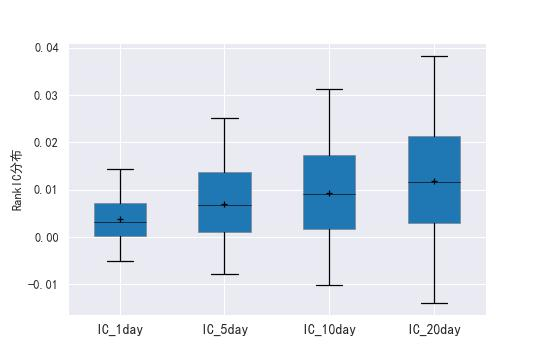
\includegraphics[width=0.9\textwidth,height=0.5\textwidth]{RankIC.jpg}
    \caption{单因子RankIC分布}
    \label{fig:rankic}
\end{figure} 

为了刻画非线性关系,Figure \ref{fig: single}展示了在我们的回测期,单个基本面因子多空组合(截面因子值最高20\%减去最低20\%)的表现状况,纵轴代表累计净值(由于仅仅考察信号的预测能力,未扣除费用)。总体上,单因子多空组合的平均净值为1.295,标准差达到0.248。可以发现,单因子表现出现分化,表现最好的因子为每股净资产、市盈率(均为每股指标)、营业收入同比增长率(成长类指标),净值分别达到1.907,1.758,1.725;表现最差的因子为股息率、应付账款周转率、管理费用/营业收入,净值为0.867,0.987,1.017。31个因子中有两个在回测期净亏损,这说明因子可能是以非线性的方式隐含的,未能被排序多空的投资组合很好地利用。因子的不同表现可能隐含着不同的信息,从而为因子组合提供了空间。

\begin{figure}[H]
    \centering
    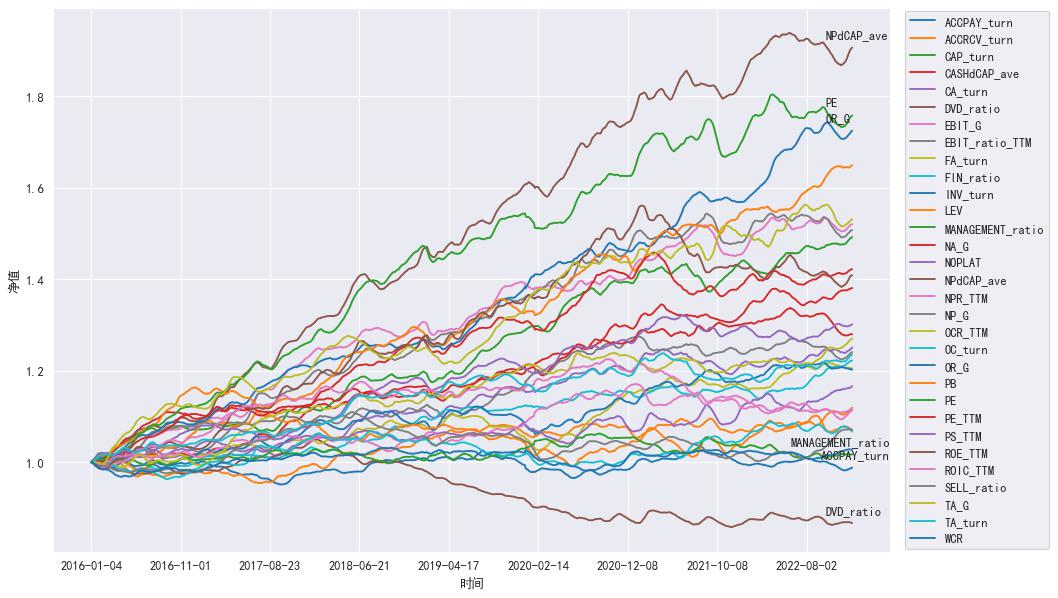
\includegraphics[width=1\textwidth,height=0.5\textwidth]{single_factor.jpg}
    \caption{单因子回测期表现}
    \label{fig: single}
\end{figure} 

兼顾风险以及收益-风险比角度,表\ref{tab: describe}进一步总结了单因子的最大回撤、夏普率、卡玛比率等指标。单因子的平均最大回撤为-7.5\%,回撤最严重的因子达到-31\%;因子总体的夏普率水平不高,为0.525;因子的卡玛比率平均达到11左右,说明因子在控制回撤下的收益较好;从胜率上看,平均胜率略高于50\%,且较为集中。


\begin{table}[H]
\centering
\caption{单因子描述性统计}
\label{tab: describe}
\begin{tabular}{cllll}
\toprule
& 最大回撤     & 夏普率    & 卡玛比率   & 胜率      \\ \midrule
均值  & -7.50\%  & 0.525  & 10.991 & 51.40\% \\
标准差 & 4.80\%   & 0.542  & 11.333 & 1.40\%  \\
最小值 & -31.00\% & -0.954 & -3.074 & 47.00\% \\
最大值 & -3.50\%  & 1.685  & 41.313 & 54.80\% \\ \bottomrule
\end{tabular}
\end{table}

\section{因子组合与策略设计}
\subsection{因子组合方式}
出于解决因子值间多重共线性,以及综合因子信号、构建更优资产组合的目的,我们尝试不同方式,将上述基本面因子综合为一个信号。查阅相关文献、研报并结合所学,我们决定通过以下7种方式进行因子组合:
\begin{enumerate}
    \item \textbf{等权法(Average)}
    
    所有因子等权重相加并重新进行标准化处理。
    \item \textbf{历史因子收益率(半衰)加权法 (HistFactorRet)}
    
    计算因子历史收益率的算数平均值或半衰加权的历史平均收益率,作为因子加权的权重;半衰加权意味着每经过半衰期H个时点(向前推H个时点),该时点的因子收益率值在加权平均中的权重减少一半。具体地,若权重为$\bm{w} = (w_1,w_2,\dots,w_N)$,$w_N$为当期权重,那么$w_t \propto 2^{\frac{t-N-1}{H}}$。
    \item \textbf{历史因子IC(半衰)加权法 (HistoryIC)}
    
    计算因子历史RankIC的算数平均值或半衰加权的历史平均RankIC,作为因子加权的权重。
    \item \textbf{最大化ICIR加权法 (MaxICIR)}
    
    ICIR等于IC的期望值除以标准差。以历史因子平均IC值作为复合因子下一期IC的估计,以历史IC值的协方差矩阵作为对复合因子下一期波动率的估计,记$\bm{w}^*=(w_1^*,w_2^*,\dots,w_N^*)$为因子合成的权重,$\bm{IC}=(\overline{IC}_1, \overline{IC}_2, \dots,\overline{IC}_N)^T$表示因子IC的均值向量,$\Sigma$为因子IC的协方差矩阵,则问题变为
$$\max ICIR=\frac{\bm{w}^T \bm{IC}}{\sqrt{\bm{w}^T \Sigma \bm{w}}}$$ 

显式解为$\bm{w}=\Sigma^{-1} \cdot \bm{IC}$,此后进行归一化处理。实际应用中,通常添加约束条件$\bm{w} \geq \bm{0}$,从而上述问题变为
$$\max ICIR=\frac{\bm{w}^T \bm{IC}}{\sqrt{\bm{w}^T \Sigma \bm{w}}}$$ $$\text{s.t. }\quad \bm{w}\geq 0$$ 
此外,本研究采用Ledoit \& Wolf (2004)\cite{ledoit2004well}给出的压缩估计方法改善对真实协方差矩阵的估计。Ledoit等人证明了改进后的协方差矩阵估计是无偏的。具体的求解数学表达式可参考附录。
\item \textbf{最大化IC加权法 (MaxIC)}

与最大化ICIR加权法的估计类似,最大化IC的加权权重同样是下列优化问题的解
$$\max IC=\frac{\bm{w}^T \bm{IC}}{\sqrt{\bm{w}^T V \bm{w}}}$$ $$\text{s.t. }\quad \bm{w}\geq 0$$ 其中相比最大化ICIR的优化方式,仅仅将$\Sigma$替换成了$V$,即当前截面因子值的相关系数矩阵。此外,我们同样对样本因子值的协方差矩阵做上述压缩估计以获得无偏估计。
\item \textbf{主成分分析估计法(PCA)}

该方式直接对所有因子进行主成分分析降维,取第一主成分作为组合后的因子值。该方式的优势是组合结果通常较为稳定,不依赖于因子收益、IC/ICIR,但与此同时也可能因未充分利用历史信息而“欠拟合”。本研究中统一取总成分数为5的降维结果的第一主成分。
\item \textbf{神经网络(DCM, Deep Correlation Model)}

\begin{enumerate}
    \item 总体思路:
    在传统使用机器学习等方式进行因子组合优化的方式中,通常将问题定义为回归问题,损失函数通常具有类似MSE的形式。也即$$Loss1=-\sum_t (y_{t+1} - f(\bm{x}_{t,i}))^2$$ 使用此类损失函数更多拟合的是$y_{t+1}$和$f(\bm{x}_{t,i})$均值之间的关系而损失了顺序信息。为此,我们考虑寻找信噪比更高的对象进行学习,将优化目标定为IC。在因子合成中,优化IC的目标函数为
$$Loss2=-\sum_t Corr(y_{t+1}, f(\bm{x}_{t,i}))$$ 其将每期的样本看做一个整体,对整体的结果计算相关性作为损失,较单一样本直接加总的损失有更高的信噪比。
由于IC描述的是整体样本的相关性,局部可能出现与整体截然相反的分布,比如整体的IC是正值,但在因子值较高的区域,IC是负值。这一结果可能会显著的影响多头选股的效果。为了更好的适应\textbf{多头选股}的任务,可采用加权的相关系数,根据因子值从高到低采用指数衰减权重
$$w_i=\left(\frac{1}{2}\right)^{\frac{i-1}{n-1}}, \quad i=1,\dots,n$$ 在上述加权的基础上,Weighted IC计算如下:
$$\mathbb{E}[x|w]=\sum_i w_i x_i, \quad \mathbb{E}[y|w]=\sum_i w_i y_i$$ $$Var[x|w]=\mathbb{E}[x^2|w]-\mathbb{E}[x|w]^2=\sum_i w_i x_i^2-\left(\sum_i w_i x_i\right)^2$$ $$Var[y|w]=\mathbb{E}[y^2|w]-\mathbb{E}[y|w]^2=\sum_i w_i y_i^2-\left(\sum_i w_i y_i\right)^2$$ $$Cov(x,y|w)=\sum_i w_i x_i y_i - \left(\sum_i w_i x_i\right)\left(\sum_i w_i y_i\right)$$ $$Corr(x,y|w)=\frac{Cov(x,y|w)}{\sqrt{Var[x|w]Var[y|w]}}$$ 使用该方法可以使得模型更关注头部(因子值较高时)的相关性。
\item 网络结构: 
考虑到输入数据的形式为横截面数据,为减轻过拟合,我们采用类似多层感知机的三层网络结构,每层分别包含一个64/128/64节点的全连接层和批次标准化层,使用ReLU函数激活。
\item 模型训练时的损失函数计算中,需将模型输出值$\hat{y}_{t+1,i}=f(\bm{x}_{t,i})$排序后计算上述加权IC值作为损失函数,从而通过反向传播更新参数,训练模型。
\end{enumerate}

\end{enumerate}

\subsection{策略方案设计}
在以上因子组合方式的基础上,我们可以从三个维度设计如表\ref{tab: combo_method}的策略方案:
\begin{table}[H]
  \centering
  \caption{策略方案设计}
    \begin{tabular}{cl}
    \toprule
    \multicolumn{1}{c}{策略维度} & 可选方案 \\
    \midrule
    \multirow{4}[2]{*}{组合因子} & 因子原始值(Origin) \\
          & 因子原始值+Barra组合(Origin+Barra) \\
          & 正交化后的残差因子(Resid) \\
          & 正交化后的残差因子+Barra组合(Resid+Barra) \\
    \hline
    \multirow{4}[2]{*}{组合的权重窗口} & \multicolumn{1}{l}{1天} \\
          & \multicolumn{1}{l}{5天} \\
          & \multicolumn{1}{l}{10天} \\
          & \multicolumn{1}{l}{20天} \\
    \hline
    \multirow{7}[2]{*}{组合方式} & 等权法 (Average)\\
          & 历史因子收益率(半衰)加权法(HistFactorRet) \\
          & 历史因子IC(半衰)加权法(HistoryIC) \\
          & 最大化ICIR加权法(MaxICIR) \\
          & 最大化IC加权法MaxIC \\
          & 主成分分析估计法(PCA) \\
          & 神经网络(DCM) \\
    \bottomrule
    \end{tabular}%
  \label{tab: combo_method}%
\end{table}

\begin{itemize}
    \item 维度1:\textbf{组合因子}。
    
    有四种可以选取的因子值作为组合的原材料:因子原始值 (Origin),因子原始值 +Barra 组合(Origin+Barra),正交化后的残差因子(Resid),正交化后的残差因子 +Barra 组合(Resid+Barra)。其中“+Barra组合”是指在原始因子的基础上再加入Barra因子值。“正交化后的残差因子”是指将原始因子对市值和行业因子做中性化后得到的残差因子。
    \item 维度2:\textbf{组合的权重窗口}
    
    可以通过更改计算组合权重的窗口来尝试不同窗口对因子表现的影响。例如,可以计算当日截面因子值和未来 1 日/ 5 日/ 10 日/ 20 日总收益率相关性(IC),来计算不同窗口期应该采用的组合权重,
    \item 维度3:\textbf{组合方式}
    
    如3.1所述,有7种组合方法。
\end{itemize}
通过对3个维度选择不同方案,我们可以得到 $4 \times 4 \times 7 = 112$个策略。
\section{策略回测} 
下面对这112个策略结果进行回测。\footnote{该部分代码参见 https://github.com/wins-m/sys23}
\subsection{回测设定与回测指标}
回测设定如下:
\begin{itemize}
    \item 股池:ST、*ST以外的全市场A股,且去除:
    \begin{itemize}
        \item T0, T-1, T-2 停牌/复牌的股票
        \item T0, T-1 涨停/跌停的股票
        \item 新上市 60 个交易日内的股票
    \end{itemize}
    \item 回测时间区间:2016-01-04至2022-12-30(样本内)
    \item 分组回测:多空 5 组
    \item IC计算的窗口:当日截面因子值和未来1日/5日/10日/20日总收益率相关性
\end{itemize}

回测的具体指标如下:
\begin{enumerate}

    \item \textbf{单位净值(Unit Value)}
    
单位净值是投资组合价值的度量,它表示每个投资单位的价值。计算方法:将投资组合的总市值除以投资单位数。单位净值有助于评估投资组合的增长,投资者可以通过单位净值观察投资组合的价值变化。
    \item \textbf{总收益率(Total Return)}
    
总收益率是投资组合在一段时间内的总回报,包括资本收益和利息收益。计算方法:将期末投资组合价值减去期初投资组合价值,然后除以期初投资组合价值。总收益率用于衡量投资组合的整体表现。

\item \textbf{最大回撤(Maximum Drawdown)}

最大回撤是指投资组合在其历史最高价值和随后的最低价值之间的最大下跌幅度。计算方法:找到历史上最大的峰值到谷值的百分比下降。最大回撤反映了投资组合在最不利情况下的损失程度,用于评估风险。

\item \textbf{夏普比率(Sharpe Ratio)}

夏普比率是用于评估投资组合的风险调整收益的指标。计算方法:将投资组合的超额收益(投资组合收益率减去无风险收益率)除以投资组合的标准差(波动性)。夏普比率越高,表示投资组合在承担相同风险的情况下,产生的超额收益越高。

\item \textbf{卡玛比率(Calmar Ratio)}

卡玛比率是另一种风险调整收益的指标,主要用于评估对冲基金和期货策略。计算方法:将年化收益率除以最大回撤。卡玛比率越高,表示投资组合在承担最大回撤风险的情况下,产生的收益越高。

\item \textbf{胜率(Win Rate)}

胜率是投资组合盈利交易次数占总交易次数的百分比。计算方法:将盈利交易次数除以总交易次数。胜率用于衡量投资组合策略的成功率,胜率越高,表示策略的预测能力越强。

\item \textbf{年化收益率(Annualized Return)}

年化收益率是指将投资组合的收益率转换为年度收益率,以便于不同投资期限的策略进行比较。较高的年化收益率意味着投资策略在长期内能够产生较高的收益。计算方法:
    \begin{enumerate}
        \item 计算投资组合的每期收益率。
        \item 将每期收益率加1,然后求积。
        \item 计算投资组合的年化几何平均收益率。假设投资期限为T年,期数为N,将上一步计算得到的积开T/N次方,然后减去1.
    \end{enumerate}
\item \textbf{信息系数IC(Information Coefficient)}

信息系数IC用于衡量因子预测能力。它是因子收益与股票收益之间的相关系数。计算方法:
    \begin{enumerate}
    \item 对每个时间截面(如每个月),计算因子值与股票未来收益的相关系数。
    \item 计算所有时间截面的平均相关系数作为IC值。
    \end{enumerate}
\item \textbf{信息比率IR(Information Ratio)}

信息比率IR,用于衡量因子表现相对于基准的超额收益。较高的IR值通常表示因子具有较强的预测能力和表现。计算方法:
    \begin{enumerate}
    \item 对每个时间截面(如每个月),计算因子组合的超额收益(组合收益减去基准收益)。
    \item 计算所有时间截面的超额收益的均值和标准差。
    \item IR = 超额收益均值 / 超额收益标准差。
    \end{enumerate}
\item \textbf{Rank IC}

类似于IC,但使用的是因子值与股票未来收益的排序之间的相关系数。计算方法如下:
    \begin{enumerate}
    \item 对每个时间截面(如每个月),计算因子值与股票未来收益的排序相关系数(即斯皮尔曼秩相关系数或肯德尔秩相关系数)。
    \item 计算所有时间截面的平均排序相关系数作为Rank IC值。
    \end{enumerate}
\item \textbf{IC IR}

类似于IR,但使用IC值代替超额收益。较高的IC IR值表示因子具有较好的稳定性。计算方法如下:
    \begin{enumerate}
    \item 对每个时间截面(如每个月),计算因子收益与股票收益之间的IC值。
    \item 计算所有时间截面的IC值的均值和标准差。
    \item IC IR = IC均值 / IC标准差。
    \end{enumerate}
\end{enumerate}


\subsection{回测效果展示}
通过4.1节中的回测设定和回测指标,我们对上面的112种策略方案都进行了回测。以部分策略为例,画出其扣除手续费后累积净值(累乘)随时间的变化,展示在图\ref{fig:factor_combo}中。



\begin{figure}[htbp]
	\begin{minipage}{0.5\linewidth}
		\centerline{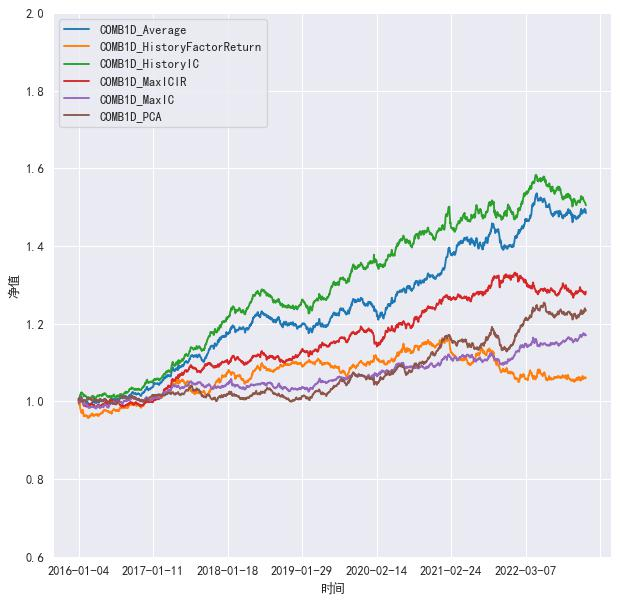
\includegraphics[width=\textwidth]{COMB.jpg}}
		\centerline{正交化后的残差因子组合}
	\end{minipage}
	\begin{minipage}{0.5\linewidth}
		\centerline{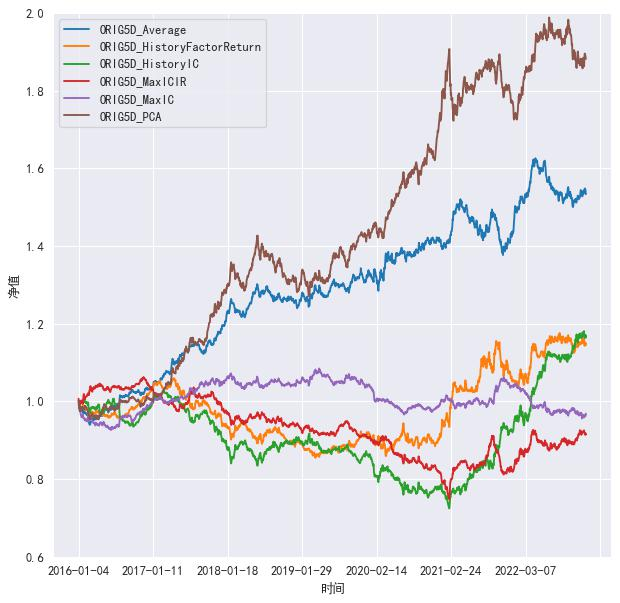
\includegraphics[width=\textwidth]{ORIG.jpg}}	 
		\centerline{因子原始值 +Barra 组合}
	\end{minipage}
 
	\caption{部分组合策略回测期表现(扣除手续费后)}
	\label{fig:factor_combo}
\end{figure}


由于变量较多,我们固定维度1(组合因子),根据夏普和收益率两个指标选择维度2(组合的权重窗口)的最优取值,再综合比较不同组合方式(维度3)下对空投资组合的表现差异。经过尝试发现,前两个维度选择方案为:\{组合因子=正交化后的残差因子(Resid),组合的权重窗口 = 1天\}\footnote{完整回测见 https://github.com/wins-m/sys23/blob/main/demo/backtest[comb1].ipynb}与\{因子原始值 +Barra 组合(Origin+Barra), 组合的权重窗口 = 5天\}\footnote{完整回测见 https://github.com/wins-m/sys23/blob/main/demo/backtest[orig5].ipynb}时,效果较好,而两种维度1的组合因子表现不佳——这非常符合我们去除 Barra 取残差这一步骤背后的经济含义。在选定前两个维度后,我们更关注不同的因子组合方式的优劣(以等权 Average 组合为对比基准),得到回测结果如表\ref{tab: comb-backtest}和表\ref{tab:ori+barra 5d backtest}。\footnote{其他所有回测过程及结果图表请通过网盘下载:https://www.aliyundrive.com/s/XGJJLKSDEXM
}

\begin{table}[htbp]
  \centering
  \captionsetup{justification=centering}
    \caption{组合因子=正交化后的残差因子(Resid),组合的权重窗口 = 1天,\\不同因子组合-回测结果展示}
    \label{tab: comb-backtest}
    \begin{tabular}{lrrrrrrr}
    \toprule
    组合方式  & \multicolumn{1}{l}{单位净值} & \multicolumn{1}{l}{总收益率} & \multicolumn{1}{l}{最大回撤} & \multicolumn{1}{l}{夏普比率} & \multicolumn{1}{l}{卡玛比率} & \multicolumn{1}{l}{胜率} & \multicolumn{1}{l}{年化收益率} \\
    \midrule
    \textbf{扣除手续费前} &       &       &       &       &       &       &  \\
    Average & 1.4111  & 41.11\% & -4.85\% & 1.5539  & 32.0081  & 53.67\% & 5.02\% \\
    PCA   & 1.2233  & 22.33\% & -5.41\% & 0.9655  & 17.8489  & 51.32\% & 2.91\% \\
    HistFactorRet & 1.0924  & 9.24\% & -9.74\% & 0.3526  & 3.6211  & 51.44\% & 1.26\% \\
    \rowcolor[rgb]{ .851,  .851,  .851} HistoryIC & 1.4290  & 42.90\% & -5.16\% & 1.5804  & 30.6535  & 53.67\% & 5.20\% \\
    MaxICIR & 1.2686  & 26.86\% & -4.81\% & 1.1330  & 23.5754  & 52.44\% & 3.44\% \\
    MaxIC & 1.2224  & 22.24\% & -2.58\% & 1.1912  & 46.1586  & 53.73\% & 2.89\%\\
    \hline
    \textbf{扣除手续费后} &       &       &       &       &       &       &  \\
    Average & 1.4004  & 40.04\% & -4.92\% & 1.5136  & 30.7460  & 53.61\% & 4.90\% \\
    PCA   & 1.2137  & 21.37\% & -5.44\% & 0.9239  & 16.9764  & 51.26\% & 2.79\% \\
    HistFactorRet & 1.0632  & 6.32\% & -10.12\% & 0.2414  & 2.3852  & 51.20\% & 0.88\% \\
    \rowcolor[rgb]{ .851,  .851,  .851} HistoryIC & 1.4143  & 41.43\% & -5.26\% & 1.5263  & 29.0312  & 53.55\% & 5.05\% \\
    MaxICIR & 1.2532  & 25.32\% & -4.95\% & 1.0675  & 21.5543  & 52.32\% & 3.26\% \\
    MaxIC & 1.1597  & 15.97\% & -3.14\% & 0.8550  & 27.2501  & 52.61\% & 2.13\% \\
    \bottomrule
    \end{tabular}%
  \label{tab:Resid1D}%
\end{table}

从表\ref{tab: comb-backtest}中可以看到,无论是在扣除手续费前还是费后,历史IC加权(HistoryIC)的组合方式的效果都是最好的。以扣除手续费后为例,回测期内年化收益率达5.05\%,最大回撤为-5.26\%,夏普比率为1.5263,卡玛比率为29.0312,胜率为53.55\%,年化收益率为5.05\%。虽然历史IC加权法(HistoryIC)最大回撤比最大化IC法(MaxIC)的-3.14\%稍大一些,但是历史IC加权(HistoryIC)的卡玛比率更大,这意味着历史IC加权组合不仅平均而言有较高的长期收益和超额收益,并且在承担最大回撤风险的情况下,产生的收益较高。

\begin{table}[htbp]
  \centering
  \captionsetup{justification=centering}
  \caption{组合因子 = 因子原始值 +Barra 组合(Origin+Barra), 组合的权重窗口 = 5天,\\ 不同因子组合-回测结果展示}
    \begin{tabular}{lrrrrrrr}
    \toprule
    组合方式  & \multicolumn{1}{l}{单位净值} & \multicolumn{1}{l}{总收益率} & \multicolumn{1}{l}{最大回撤} & \multicolumn{1}{l}{夏普比率} & \multicolumn{1}{l}{卡玛比率} & \multicolumn{1}{l}{胜率} & \multicolumn{1}{l}{年化收益率}\\
    \midrule
    \textbf{扣除手续费前} &       &       &       &       &       &       &  \\
    Average & 1.4491  & 44.91\% & -9.68\% & 1.1191  & 11.5661  & 52.44\% & 5.41\% \\
    \rowcolor[rgb]{ .851,  .851,  .851} PCA   & 1.6584  & 65.84\% & -11.34\% & 1.3742  & 12.1150  & 53.55\% & 7.45\% \\
    HistFactorRet & 1.1839  & 18.39\% & -20.46\% & 0.3510  & 1.7159  & 50.38\% & 2.43\% \\
    HistoryIC & 1.1958  & 19.58\% & -33.03\% & 0.3678  & 1.1137  & 50.62\% & 2.57\% \\
    MaxICIR & 0.9400  & -6.00\% & -33.42\% & -0.1512  & -0.4524  & 48.62\% & -0.88\% \\
    MaxIC & 0.9979  & -0.21\% & -11.11\% & -0.0074  & -0.0667  & 50.09\% & -0.03\% \\
    \hline
    \textbf{扣除手续费后} &       &       &       &       &       &       &  \\
    Average & 1.4392  & 43.92\% & -9.77\% & 1.0947  & 11.2079  & 52.38\% & 5.31\% \\
    \rowcolor[rgb]{ .851,  .851,  .851} PCA   & 1.6490  & 64.90\% & -11.43\% & 1.3546  & 11.8493  & 53.44\% & 7.37\% \\
    HistFactorRet & 1.1546  & 15.46\% & -21.15\% & 0.2951  & 1.3954  & 50.21\% & 2.06\% \\
    HistoryIC & 1.1724  & 17.24\% & -34.12\% & 0.3239  & 0.9492  & 50.50\% & 2.29\% \\
    MaxICIR & 0.9223  & -7.77\% & -34.62\% & -0.1959  & -0.5657  & 48.62\% & -1.14\% \\
    MaxIC & 0.9741  & -2.59\% & -12.33\% & -0.0906  & -0.7349  & 49.85\% & -0.37\% \\
    \bottomrule
    \end{tabular}%
  \label{tab:ori+barra 5d backtest}%
\end{table}%

从表\ref{tab:ori+barra 5d backtest}中可以看到,如果采用原始的因子值和 Barra 风格因子一起进行组合,则 PCA 组合方式的综合表现最好。以扣除手续费后为例,回测期内年化收益率高达 7.37\%,夏普比率为 1.3546,卡玛比率为11.85,胜率为53.44\%。除了 PCA 组合方式以及作为基准的等权组合方式(Average)以外,其他组合方式的表现则相当一般。

对比表\ref{tab: comb-backtest}和表\ref{tab:ori+barra 5d backtest}的结果,我们也会发现加入 Barra 风格因子后进行组合所构建的投资组合普遍体现更高的回撤、更低的夏普以及更低的卡玛比率。这可能说明,引入 Barra 会带来更多的 beta 噪音而非 alpha 信息,使得组合时过多地对权重窗口期内的噪声进行了拟合,而不能很好地预见未来的信息;PCA 能够通过矩阵特征值分解的方法提取出噪音信号中的有效信息,因此表现较好;由于 31 个含有 alpha 信息的基本面因子占多数,因子直接等权组合的表现也相对稳健。

综合来看,直接用正交化后的残差因子进行组合的方式更能够得到比较稳健的投资策略,而用因子原始值和 Barra 风格因子进行组合则可以获得一定的 beta 暴露,从而获得激进型的高额收益,这一结果同样说明了学术界和业界使用 beta / alpha 的因子划分并采用 Barra 模型等方法控制风险的科学性。为了便于比较,将原始因子和正交化后的残差因子(Resid)扣除手续费后的回测结果列在附录中的表\ref{tab:raw factor}和表\ref{tab:resid}中。通过比较可以发现,虽然诸如NPdCAP\_ave(平均每股净资产)等单因子可能已经取得了较高的收益率,但组合后的因子相较原始因子仍有较多维度的表现提升。表\ref{tab:ori+barra 5d backtest}中效果最好的组合方式(PCA),在收益率上更进一步:年化收益率从单个因子的7.15\%提升到了7.45\%。最大回撤从单因子的-9.13\%增加到-11.43\%,在可接受的范围内。夏普比率、胜率也基本持平。这说明我们的因子组合策略有着比单因子策略更好的效果。


\section{总结与展望}
本文通过构建基本面因子,回测单因子的表现,尝试多种因子组合方式,并从三个维度(组合因子维度,组合的权重窗口维度,组合方式维度)构建了112种合成方式和多空策略,在A股全市场进行为期7年的回测。通过年化收益率、最大回撤、夏普比率、卡玛比率、胜率等指标筛选出其中效果较好的策略,如表\ref{tab:strategy}所示:

\begin{table}[H]
  \centering
  \caption{两个较优策略方案}
    \begin{tabular}{p{6.585em}ccccccc}
    \toprule
    \multicolumn{1}{l}{策略方案} & \multicolumn{1}{l}{单位净值} & \multicolumn{1}{l}{总收益率} & \multicolumn{1}{l}{最大回撤} & \multicolumn{1}{l}{夏普比率} & \multicolumn{1}{l}{卡玛比率} & \multicolumn{1}{l}{胜率} & \multicolumn{1}{l}{年化收益率}\\
    \midrule
    \multicolumn{1}{l}{\textbf{扣除手续费前}} &       &       &       &       &       &       &  \\
    稳健型策略   & 1.4290 & 42.90\% & -5.16\% & 1.5804 & 30.6535 & 53.67\% & 5.20\% \\
    进取型策略   & 1.6584 & 65.84\% & -11.34\% & 1.3742 & 12.115 & 53.55\% & 7.45\% \\
    \hline
    \multicolumn{1}{l}{\textbf{扣除手续费后}} &       &       &       &       &       &       &  \\
    稳健型策略   & 1.4143 & 41.43\% & -5.26\% & 1.5263 & 29.0312 & 53.55\% & 5.05\% \\
    进取型策略   & 1.6490 & 64.90\% & -11.43\% & 1.3546 & 11.8493 & 53.44\% & 7.37\% \\
    \bottomrule
    \end{tabular}%
  \label{tab:strategy}%
\end{table}%

其中稳健型策略和进取型策略的具体配置方案如表\ref{tab:strategyinfo}所示。

\begin{table}[H]
  \centering
  \caption{策略配置方案概览}
    \begin{tabular}{cll}
    \toprule
    \multicolumn{1}{l}{策略种类} & 组合维度  & 选择方案 \\
    \midrule
    \multirow{3}[2]{*}{稳健型策略} & 组合因子 & 正交化后的残差因子(Resid) \\
          & 组合的权重窗口 & 1天 \\
          & 组合方法  & 历史因子IC(半衰)加权法(HistoryIC)\\
    \hline
    \multirow{3}[2]{*}{进取型策略} & 组合因子 & 因子原始值+Barra组合(Origin+Barra)\\
          & 组合的权重窗口 & 5天 \\
          & 组合方法  & 主成分分析估计法(PCA) \\
    \bottomrule
    \end{tabular}%
  \label{tab:strategyinfo}%
\end{table}%

由表\ref{tab:strategy}可知,
\begin{itemize}
    \item 稳健型策略在扣除手续费前的总收益率为42.90\%,年化收益率为5.20\%,最大回撤为-5.16\%,夏普比率为1.5804,卡玛比率为30.6535,胜率为53.67\%。扣除手续费后,总收益率略有下降至41.43\%,年化收益率为5.05\%,最大回撤稍微增加至-5.26\%,夏普比率为1.5263,卡玛比率为29.0312,胜率为53.55\%。从这些指标来看,稳健型策略的整体表现较为稳定,风险相对较低,适合风险厌恶的投资者。
    \item 进取型策略在扣除手续费前的总收益率为65.84\%,年化收益率为7.45\%,最大回撤为-11.34\%,夏普比率为1.3742,卡玛比率为12.115,胜率为53.55\%。扣除手续费后,总收益率略有下降至64.90\%,年化收益率为7.37\%,最大回撤稍微增加至-11.43\%,夏普比率为1.3546,卡玛比率为11.8493,胜率为53.44\%。相较于稳健型策略,进取型策略的收益率更高,但同时承担了更高的风险,适合风险承受能力较强的投资者。
    \item 通过将表\ref{tab:strategy}与表\ref{tab:raw factor}和表\ref{tab:resid}中原始因子和正交化后的残差因子 (Resid) 的回测结果对比可以发现,年化收益率有所提高,最大回撤略有增加,夏普比率、胜率也基本持平。这说明我们的因子组合策略有着比单因子策略更好的效果。
\end{itemize}

综上所述,稳健型策略和进取型策略各有优缺点,投资者可以根据自己的风险承受能力、投资目标和投资期限来选择适合自己的策略。在实际操作中,投资者可以进一步优化策略,例如调整因子权重、优化组合方法等,以期在控制风险的同时提高收益率。



\section{附录}
\begin{enumerate}
  \item \textbf{因子组合中的半衰加权公式}:设半衰期参数为$H$,过去共有$T$期数据,加权权重$w=(w_1,w_2,\dots,w_t)$, $w_1$是距离现在最远的一期权重。则有初始$w_t$
  $$w_t=2^{\frac{t-T-1}{H}}, \quad t=1,2,\dots,T$$ 在实际操作中,需对上述权重进行归一化:
  $$w_t'=\frac{w_t}{\sum w_t}$$
  此方法可应用到历史IC加权组合,历史因子收益率加权组合等方式中,以提升近期因子表现的权重。本研究中,统一取$T=250,H=50$,即250个交易日历史数据(约1年)进行加权,权重每50个交易日变为原先的一半。
  \item 为使得加权结果稳定,在\textbf{因子组合模块}中使用的所有IC均为RankIC而非常规的PearsonIC。
  \item \textbf{协方差矩阵的压缩估计。} 设$\Sigma^*$是对真实协方差矩阵$\Sigma$在有限样本下的渐进一致估计,$S$是样本$X$的协方差矩阵,则需要找到$\Sigma^*$,使得
  $$\mathbb{E}\left[\|\Sigma^*-\Sigma\|^2\right]$$
  尽可能小,其中$\|\cdot\|$是矩阵的Frobenius范数(即所有元素的均方根),也即
  $$\|A\|=\sqrt{tr(AA^T)/N}$$
  Ledoit和Wolf证明了对于样本$X=(x_t)$和其协方差矩阵$S(N\times T)$,该问题的压缩估计为
  $$\Sigma^*=\rho_1 I+\rho_2 S$$
  其中
  $$\rho_1=\frac{b^2}{d^2}m, \quad \rho_2=\frac{a^2}{d^2}$$
  $$m=\|S-I\|^2, \quad d^2=\|S-mI\|^2, \quad b_0^2=\frac{1}{T^2}\sum_{t=1}^T \|x_t \cdot x_t^T-S\|^2$$
  $$b^2=\min(b_0^2,d^2), \quad a^2=d^2-b^2$$
  此方法应用在因子优化中,最大化IC和ICIR的组合方式的协方差矩阵估计中。
  \item 因子优化的一种较为复杂的方式:\textbf{最小波动因子组合法}。本方法由Menchero \& Lee (2015) \cite{menchero2015efficiently}提出,由于涉及较为复杂的股票收益协方差矩阵计算,在本研究中因算力限制暂未实现,可供参考。最小波动因子组合是\textbf{所有在目标因子上具有单位暴露的组合中,预期风险最小的组合}。其权重根据马科维茨均值-方差模型优化得到:
  $$\min_w w'Vw$$ $$\text{s.t. }w'X_k=1$$ 上述优化问题有显式解
  $$\Omega_k^{MV}=\frac{V^{-1}X_k}{X_k'V^{-1}X_k}$$
  
  在所有的因子组合中,最小波动因子组合是在单位目标因子暴露的条件下预期风险最小的组合,因此其夏普比率在理论上来讲是最高的。我们考虑将对$K$个因子的配置问题转化为对$K$个最小波动因子组合的配置问题。假设我们有$K$个Alpha因子,股票$n$在因子$k$上的暴露为$X_{nk}^{(\alpha)}$,则构建的复合因子为
  $$\alpha_n=\sum_{k=1}^K v_k X_{nk}^{(\alpha)}$$ 根据马科维茨的期望-方差模型,根据该复合因子$\bm{\alpha}$构建出的最小波动因子组合的权重为
  $$h=\frac{V^{-1}\bm{\alpha}}{\bm{\alpha}'V^{-1}\bm{\alpha}}$$ 式中$V (N\times N)$为个股收益率的协方差矩阵。令
  $$\lambda =\bm{\alpha}'V^{-1}\bm{\alpha} $$ 将$\bm{\alpha}$用多个Alpha的线性组合替代,得到
  $$h=\frac{1}{\lambda}\left[\sum_{k=1}^K v_k V^{-1}\bm{X}_k^{(\alpha)} \right]$$ 对于单个Alpha因子$k$,参考上文中的推导,其对应的最小波动因子组合个股权重$h_k$满足
  $$h_k=\frac{V^{-1}X_k^{(\alpha)}}{s_k}, \quad s_k=X_k^{'(\alpha)}V^{-1}X_k^{(\alpha)}$$ 也即上述模型的单个向量形式。比较$h$和$h_k$,我们有
  $$h=\frac{1}{\lambda}\left[\sum_{k=1}^K v_k s_k h_k \right]=\sum_{k=1}^K w_k h_k$$ 其中
  $$w_k=\frac{1}{\lambda} v_k s_k$$ 从而因子组合的加权权重$v_k$依赖于多个因子的最小波动组合资产配置权重$w_k$:
  $$v_k=\frac{\lambda w_k}{s_k}$$ 我们考虑由这$K$个最小波动组合“资产”的协方差矩阵$G$,其每个元素可表示为
  $$G=(G_{kl})=(h_k' V h_l)$$ 其中,$G_{kl}$表示因子$k$和因子$l$的最小波动组合收益率协方差,$V$为个股协方差$(N\times N)$。因子$k$的最小波动组合的预期收益应当为其在个股上的权重与对应个股期望收益率的乘积。$$\alpha_k^{MV}=\sum_{m=1}^N \Omega_{km}^{MV}\alpha_m^P$$ 其中$\alpha_m^P$为个股期望收益率,而$\Omega_{km}$的显式解见上文的优化问题。

  综上所述,我们可以得到最优配置权重$w$:
  $$w=\frac{1}{\lambda}G^{-1}\alpha^{MV}=\frac{1}{\lambda} (h'Vh)^{-1}\alpha^{MV}$$
\end{enumerate}

\begin{table}[htbp]
  \centering
  \caption{原始因子扣除手续费后回测结果(按总收益率从高到低排序)}
    \begin{tabular}{lrrrrrrr}
    \toprule
    因子名称  & \multicolumn{1}{l}{单位净值} & \multicolumn{1}{l}{总收益率} & \multicolumn{1}{l}{最大回撤} & \multicolumn{1}{l}{夏普比率} & \multicolumn{1}{l}{卡玛比率} & \multicolumn{1}{l}{胜率} & \multicolumn{1}{l}{年化收益率} \\
    \midrule
    NPdCAP\_ave & 1.6259  & 62.59\% & -9.13\% & 1.4823  & 16.2430  & 53.73\% & 7.15\% \\
    ROE\_TTM & 1.5216  & 52.16\% & -8.97\% & 1.2364  & 13.7904  & 53.79\% & 6.15\% \\
    CAP\_turn & 1.4339  & 43.39\% & -8.34\% & 1.2182  & 14.6094  & 53.85\% & 5.25\% \\
    PE    & 1.3868  & 38.68\% & -12.19\% & 0.9417  & 7.7273  & 53.02\% & 4.76\% \\
    EBIT\_G & 1.3799  & 37.99\% & -9.32\% & 1.1647  & 12.5020  & 53.26\% & 4.68\% \\
    CA\_turn & 1.3723  & 37.23\% & -9.64\% & 1.1063  & 11.4805  & 53.85\% & 4.60\% \\
    EBIT\_ratio\_TTM & 1.3403  & 34.03\% & -10.84\% & 0.9827  & 9.0633  & 51.61\% & 4.25\% \\
    TA\_turn & 1.3308  & 33.08\% & -7.79\% & 1.0003  & 12.8447  & 52.73\% & 4.14\% \\
    NPR\_TTM & 1.3060  & 30.60\% & -7.15\% & 0.9488  & 13.2643  & 52.38\% & 3.87\% \\
    OR\_G & 1.2951  & 29.51\% & -10.32\% & 0.8660  & 8.3915  & 52.20\% & 3.74\% \\
    NP\_G & 1.2925  & 29.25\% & -10.44\% & 0.8248  & 7.8968  & 52.67\% & 3.71\% \\
    ROIC\_TTM & 1.2905  & 29.05\% & -9.63\% & 0.7656  & 7.9519  & 51.61\% & 3.69\% \\
    NOPLAT & 1.2737  & 27.37\% & -13.60\% & 0.5903  & 4.3411  & 52.08\% & 3.50\% \\
    ACCRCV\_turn & 1.2504  & 25.04\% & -10.95\% & 0.5673  & 5.1793  & 53.55\% & 3.23\% \\
    FIN\_ratio & 1.2452  & 24.52\% & -8.15\% & 0.7499  & 9.2001  & 52.79\% & 3.17\% \\
    TA\_G & 1.2222  & 22.22\% & -11.46\% & 0.5523  & 4.8201  & 50.44\% & 2.89\% \\
    PE\_TTM & 1.2200  & 22.00\% & -15.91\% & 0.5075  & 3.1895  & 51.03\% & 2.87\% \\
    OC\_turn & 1.2094  & 20.94\% & -6.13\% & 0.6914  & 11.2810  & 51.38\% & 2.74\% \\
    CASHdCAP\_ave & 1.2027  & 20.27\% & -7.58\% & 0.6832  & 9.0151  & 52.91\% & 2.66\% \\
    OCR\_TTM & 1.1963  & 19.63\% & -14.41\% & 0.4822  & 3.3467  & 49.85\% & 2.58\% \\
    MANAGE\_ratio & 1.1890  & 18.90\% & -10.75\% & 0.4952  & 4.6059  & 53.20\% & 2.49\% \\
    FA\_turn & 1.1674  & 16.74\% & -8.55\% & 0.5284  & 6.1820  & 52.79\% & 2.22\% \\
    LEV   & 1.1562  & 15.62\% & -10.88\% & 0.4260  & 3.9155  & 51.20\% & 2.08\% \\
    SELL\_ratio & 1.1190  & 11.90\% & -15.02\% & 0.2392  & 1.5931  & 50.50\% & 1.61\% \\
    ACCPAY\_turn & 1.0968  & 9.68\% & -10.44\% & 0.2947  & 2.8228  & 48.33\% & 1.32\% \\
    INV\_turn & 1.0796  & 7.96\% & -11.95\% & 0.2387  & 1.9976  & 50.56\% & 1.09\% \\
    PS\_TTM & 1.0384  & 3.84\% & -26.27\% & 0.0790  & 0.3008  & 49.27\% & 0.54\% \\
    DVD\_ratio & 1.0007  & 0.07\% & 0.00\% & 0.5261  & \multicolumn{1}{r}{inf} & 0.12\% & 0.01\% \\
    FEE\_ratio & 0.9946  & -0.54\% & -12.46\% & -0.0125  & -0.1004  & 51.61\% & -0.08\% \\
    WCR   & 0.9148  & -8.52\% & -24.96\% & -0.1972  & -0.7898  & 49.27\% & -1.26\% \\
    PB    & 0.8416  & -15.84\% & -43.65\% & -0.2693  & -0.6169  & 47.97\% & -2.42\% \\
    NA\_G & 0.7885  & -21.15\% & -31.67\% & -0.6142  & -1.9397  & 48.09\% & -3.32\% \\
    \bottomrule
    \end{tabular}%
  \label{tab:raw factor}%
\end{table}%

\begin{table}[htbp]
  \centering
  \caption{正交化后的残差因子(Resid)扣除手续费后回测结果 (按总收益率从高到低排序)}
    \begin{tabular}{lrrrrrrr}
    \toprule
    因子名称  & \multicolumn{1}{l}{单位净值} & \multicolumn{1}{l}{总收益率} & \multicolumn{1}{l}{最大回撤} & \multicolumn{1}{l}{夏普比率} & \multicolumn{1}{l}{卡玛比率} & \multicolumn{1}{l}{胜率} & \multicolumn{1}{l}{年化收益率} \\
    \midrule
    NPdCAP\_ave\ & 1.4492  & 44.92\% & -4.51\% & 1.6853  & 37.3427  & 54.79\% & 5.41\% \\
    ROE\_TTM\ & 1.3558  & 35.58\% & -6.19\% & 1.1653  & 18.8238  & 53.38\% & 4.42\% \\
    CAP\_turn\ & 1.3525  & 35.25\% & -3.63\% & 1.4992  & 41.3126  & 54.02\% & 4.38\% \\
    EBIT\_G\ & 1.2638  & 26.38\% & -4.86\% & 1.2047  & 24.7763  & 52.55\% & 3.38\% \\
    PE\ & 1.2582  & 25.82\% & -6.97\% & 1.0222  & 14.6619  & 52.32\% & 3.32\% \\
    OR\_G\ & 1.2393  & 23.93\% & -4.07\% & 1.0948  & 26.9165  & 52.03\% & 3.10\% \\
    PB\ & 1.1862  & 18.62\% & -3.46\% & 0.9171  & 26.5399  & 51.79\% & 2.46\% \\
    TA\_G\ & 1.1849  & 18.49\% & -7.28\% & 0.7223  & 9.9200  & 50.91\% & 2.44\% \\
    OCR\_TTM\ & 1.1832  & 18.32\% & -3.61\% & 0.7944  & 22.0116  & 51.97\% & 2.42\% \\
    PE\_TTM\ & 1.1803  & 18.03\% & -5.05\% & 0.7787  & 15.4089  & 51.15\% & 2.38\% \\
    TA\_turn\ & 1.1684  & 16.84\% & -4.02\% & 0.7681  & 19.1027  & 52.50\% & 2.24\% \\
    INV\_turn\ & 1.1599  & 15.99\% & -7.44\% & 0.6213  & 8.3451  & 51.79\% & 2.13\% \\
    NA\_G\ & 1.1597  & 15.97\% & -4.16\% & 0.7109  & 17.1011  & 52.50\% & 2.13\% \\
    EBIT\_ratio\_TTM\ & 1.1560  & 15.60\% & -10.64\% & 0.6381  & 5.9961  & 51.32\% & 2.08\% \\
    CASHdCAP\_ave\ & 1.1462  & 14.62\% & -4.95\% & 0.6046  & 12.2139  & 52.03\% & 1.96\% \\
    ACCRCV\_turn\ & 1.1422  & 14.22\% & -5.77\% & 0.5784  & 10.0153  & 50.79\% & 1.91\% \\
    CA\_turn\ & 1.1412  & 14.12\% & -6.98\% & 0.5846  & 8.3754  & 52.44\% & 1.89\% \\
    NP\_G\ & 1.1328  & 13.28\% & -5.42\% & 0.5573  & 10.2882  & 51.32\% & 1.79\% \\
    NOPLAT\ & 1.1315  & 13.15\% & -10.05\% & 0.3849  & 3.8282  & 50.21\% & 1.77\% \\
    ROIC\_TTM\ & 1.1094  & 10.94\% & -7.32\% & 0.4590  & 6.2695  & 51.38\% & 1.49\% \\
    PS\_TTM\ & 1.1073  & 10.73\% & -4.99\% & 0.5044  & 10.0985  & 52.50\% & 1.46\% \\
    FIN\_ratio\ & 1.0883  & 8.83\% & -8.66\% & 0.4449  & 5.1391  & 50.73\% & 1.21\% \\
    NPR\_TTM\ & 1.0846  & 8.46\% & -10.49\% & 0.3499  & 3.3359  & 51.15\% & 1.16\% \\
    SELL\_ratio\ & 1.0841  & 8.41\% & -7.84\% & 0.3777  & 4.8160  & 51.97\% & 1.15\% \\
    MANAGE\_ratio\ & 1.0434  & 4.34\% & -7.93\% & 0.1822  & 2.2967  & 50.15\% & 0.61\% \\
    OC\_turn\ & 0.9947  & -0.53\% & -6.68\% & -0.0252  & -0.3767  & 50.56\% & -0.08\% \\
    ACCPAY\_turn\ & 0.9836  & -1.64\% & -10.12\% & -0.0719  & -0.7109  & 50.38\% & -0.23\% \\
    WCR\ & 0.9797  & -2.03\% & -5.36\% & -0.0997  & -1.8595  & 51.03\% & -0.29\% \\
    DVD\_ratio\ & 0.9705  & -2.95\% & -9.15\% & -0.1640  & -1.7930  & 50.21\% & -0.42\% \\
    FA\_turn\ & 0.9452  & -5.48\% & -9.01\% & -0.2571  & -2.8546  & 49.32\% & -0.80\% \\
    FEE\_ratio\ & 0.9352  & -6.48\% & -11.28\% & -0.2899  & -2.5694  & 49.91\% & -0.95\% \\
    LEV\ & 0.7564  & -24.36\% & -31.03\% & -0.9538  & -3.0740  & 47.03\% & -3.89\% \\
    \bottomrule
    \end{tabular}%
  \label{tab:resid}%
\end{table}%

\bibliographystyle{plain}
\nocite{*}
\bibliography{ref.bib}
\end{document}